%# -*- coding: utf-8 -*-
%!TEX encoding = UTF-8 Unicode
%!TEX TS-program = xelatex
% vim:ts=4:sw=4
%
% 以上设定默认使用 XeLaTex 编译,并指定 Unicode 编码,供 TeXShop 自动识别

%第六十二回 
\chapter{潘道士法遣黃巾士 西門慶大哭李瓶兒}

詩曰:

玉釵重合兩無緣,魚在深潭鶴在天。
得意紫鸞休舞鏡,傳言青鳥罷銜箋。
金盆已覆難收水,玉軫長籠不續弦。
若向蘼蕪山下過,遙將紅淚灑窮泉。

話說西門慶見李瓶兒服藥無效,求神問卜發課,皆有凶無吉,無法可處。初時,李瓶兒還
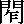
\includegraphics{figures-char/image00571.jpeg}%【門乍】
著梳頭洗臉,下炕來坐凈桶,次後漸漸飲食減少,形容消瘦,那消幾時,把個花朵般人兒,瘦弱得黃葉相似,也不起炕了,只在床褥上鋪墊草紙。恐怕人嫌穢惡,教丫頭只燒著香。西門慶見他胳膊兒瘦得銀條相似,只守著在房內哭泣,衙門中隔日去走一走。李瓶兒道:「我的哥,你還往衙門中去,只怕誤了你公事。我不妨事,只吃下邊流的虧,若得止住了,再把口裡放開,吃些飲食兒,就好了。你男子漢,常絆在我房中做甚麼!」西門慶哭道:「我的姐姐,我見你不好,心中舍不的你。」李瓶兒道:「好傻子,只不死,死將來你攔的住那些!」又道:「我有句話要對你說:我不知怎的,但沒人在房裡,心中只害怕,恰似影影綽綽有人在跟前一般。夜裡要便夢見他,拿刀弄杖,和我廝嚷,孩子也在他懷裡。我去奪,反被他推我一交,說他又買了房子,來纏了好幾遍,只叫我去。只不好對你說。」西門慶聽了說道:「人死如燈滅,這幾年知道他往那裡去了!此是你病的久,神虛氣弱了,那裡有甚麼邪魔魍魎、家親外祟!我如今往吳道官廟裡,討兩道符來,貼在房門上,看有邪祟沒有。」

說畢,走到前邊,即差玳安騎頭口往玉皇廟討符去。走到路上,迎見應怕爵和謝希大,忙下頭口。伯爵因問:「你往那裡去?你爹在家裡?」玳安道:「爹在家裡,小的往玉皇廟討符去。」伯爵與謝希大到西門慶家,因說道:「謝子純聽見嫂子不好,唬了一跳,敬來問安。」西門慶道:「這兩日身上瘦的通不象模樣了,丟的我上不上,下不下,卻怎生樣的?」伯爵道:「哥,你使玳安往廟裡做甚麼去?」西門慶悉把李瓶兒害怕之事告訴一遍:「只恐有邪祟,教小廝討兩道符來鎮壓鎮壓。」謝希大道:「哥,此是嫂子神氣虛弱,那裡有甚麼邪祟!」伯爵道:「哥若遣邪也不難,門外五嶽觀潘道士,他受的是天心五雷法,極遣的好邪,有名喚著潘捉鬼,常將符水救人。哥,你差人請他來,看看嫂子房裡有甚邪祟,他就知道。你就教他治病,他也治得。」西門慶道:「等討了吳道官符來看,在那裡住?沒奈何,你就領小廝騎了頭口,請了他來。」伯爵道:「不打緊,等我去。天可憐見嫂子好了,我就頭著地也走。」說了一回話,伯爵和希大起身去了。

玳安兒討了符來,貼在房中。晚間李瓶兒還害怕,對西門慶說:「死了的,他剛纔和兩個人來拿我,見你進來,躲出去了。」西門慶道:「你休信邪,不妨事。昨日應二哥說,此是你虛極了。他說門外五嶽觀有個潘道士,好符水治病,又遣的好邪,我明日早教應伯爵去請他來看你,有甚邪祟,教他遣遣。」李瓶兒道:「我的哥哥,你請他早早來,那廝他剛纔發恨而去,明日還來拿我哩!你快些使人請去。」西門慶道:「你若害怕,我使小廝拿轎子接了吳銀兒,和你做兩日伴兒。」李瓶兒搖頭兒說:「你不要叫他,只怕誤了他家裡勾當。」西門慶道:「叫老馮來伏侍你兩日兒如何?」李瓶兒點頭兒。這西門慶一面使來安,往那邊房子里叫馮媽媽,又不在,鎖了門出去了。對一丈青說下:「等他來,好歹教他快來宅內,六娘叫他哩。」西門慶一面又差下玳安:「明日早起,你和應二爹往門外五嶽觀請潘道士去。」俱不在話下。

次日,只見王姑子挎著一盒兒粳米、二十塊大乳餅、一小盒兒十香瓜茄來看。李瓶兒見他來,連忙教迎春搊扶起來坐的。王姑子道了問訊,李瓶兒請他坐下,道:「王師父,你自印經時去了,影邊兒通不見你。我恁不好,你就不來看我看兒?」王姑子道:「我的奶奶,我通不知你不好,昨日大娘使了大官兒到庵里,我才曉得。又說印經哩,你不知道,我和薛姑子老淫婦合了一場好氣。與你老人家印了一場經,只替他趕了網兒。背地裡和印經的打了五兩銀子夾帳,我通沒見一個錢兒。你老人家作福,這老淫婦到明日墮阿鼻地獄!為他氣的我不好了,把大娘的壽日都誤了,沒曾來。」李瓶兒道:「他各人作業,隨他罷,你休與他爭執了。」王姑子道:「誰和他爭執甚麼。」李瓶兒道:「大娘好不惱你哩,說你把他受生經都誤了。」王姑子道:「我的菩薩,我雖不好,敢誤了他的經?──在家整誦了一個月,昨日圓滿了,今日才來。先到後邊見了他,把我這些屈氣告訴了他一遍。我說,不知他六娘不好,沒甚麼,這盒粳米和些十香爪、幾塊乳餅,與你老人家吃粥兒。大娘才叫小玉姐領我來看你老人家。」小玉打開盒兒,李瓶兒看了說道:「多謝你費心。」王姑子道:「迎春姐,你把這乳餅就蒸兩塊兒來,我親看你娘吃些粥兒。」迎春一面收下去了。李瓶兒吩咐迎春:「擺茶來與王師父吃。」王姑子道:「我剛纔後邊大娘屋裡吃了茶,煎些粥來,我看著你吃些。」

:「我的菩薩,你老人家忒多慮了。你好心人,龍天自然加護。」正說著,只見琴童兒進來對迎春說:「爹吩咐把房內收拾收拾,花大舅便進來看娘,在前邊坐著哩。」王姑子便起身說道:「我且往後邊去走走。」李瓶兒道:「王師父,你休要去了,與我做兩日伴兒,我還和你說話哩。」王姑子道:「我的奶奶,我不去。」

不一時,西門慶陪花大舅進來看問,見李瓶兒睡在炕上不言語,花子由道:「我不知道,昨日聽見這邊大官兒去說,才曉的。明日你嫂子來看你。」那李瓶兒只說了一聲:「多有起動。」就把面朝里去了。花子由坐了一回,起身到前邊,向西門慶說道:「俺過世老公公在廣南鎮守,帶的那三七藥,曾吃了不曾?不拘婦女甚崩漏之疾,用酒調五分末兒,吃下去即止。大姐他手裡曾收下此藥,何不服之?」西門慶道:「這藥也吃過了。昨日本縣胡大尹來拜,我因說起此疾,他也說了個方兒:棕炭與白雞冠花煎酒服之。只止了一日,到第二日,流的比常更多了。」花子由道:「這個就難為了。姐夫,你早替他看下副板兒,預備他罷。明日教他嫂子來看他。」說畢,起身去了。

奶子與迎春正與李瓶兒墊草紙在身底下,只見馮媽媽來到,向前道了萬福。如意兒道:「馮媽媽貴人,怎的不來看看娘?昨日爹使來安兒叫你去,說你鎖著門,往那裡去來?」馮婆子道:「說不得我這苦。成日往廟裡修法,早晨出去了,是也直到黑,不是也直到黑來家,偏有那些張和尚、李和尚、王和尚。」如意兒道:「你老人家怎的有這些和尚?早時沒王師父在這裡?」那李瓶兒聽了,微笑了一笑兒,說道:「這媽媽子,單管只撒風。」如意兒道:「馮媽媽,叫著你還不來!娘這幾日,粥兒也不吃,只是心內不耐煩,你剛纔來到,就引的娘笑了一笑兒。你老人家伏侍娘兩日,管情娘這病就好了。」馮媽媽道:「我是你娘退災的博士!」又笑了一回。因向被窩裡摸了摸他身上,說道:「我的娘,你好些兒也罷了!」又問:「坐榪子還下的來?」迎春道:「下的來倒好!前兩遭,娘還��,俺每搊扶著下來。這兩日通只在炕上鋪墊草紙,一日兩三遍。」

正說著,只見西門慶進來,看見馮媽媽,說道:「老馮,你也常來這邊走走,怎的去了就不來?」婆子道:「我的爺,我怎不來?這兩日腌菜的時候,掙兩個錢兒,腌些菜在屋裡,遇著人家領來的業障,好與他吃。不然,我那討閑錢買菜來與他吃?」西門慶道:「你不對我說,昨日俺莊子上起菜,撥兩三畦與你也夠了。」婆子道:「又敢纏你老人家。」說畢,過那邊屋裡去了。

西門慶便坐在炕沿上,迎春在旁熏爇芸香。西門慶便問:「你今日心裡覺怎樣?」又問迎春:「你娘早晨吃些粥兒不曾?」迎春道:「吃的倒好!王師父送了乳餅,蒸來,娘只咬了一些兒,呷了不上兩口粥湯,就丟下了。」西門慶道:「應二哥剛纔和小廝門外請那潘道士,又不在了。明日我教來保再請去。」李瓶兒道:「你上緊著人請去,那廝,但合上眼,只在我跟前纏。」西門慶道:「此是你神弱了,只把心放正著,休要疑影他。請他來替你把這邪崇遣遣,再服他些藥,管情你就好了。」李瓶兒道:「我的哥哥,奴已是得了這個拙病,那裡好甚麼!奴指望在你身邊團圓幾年,也是做夫妻一場,誰知到今二十七歲,先把冤家死了,奴又沒造化,這般不得命,拋閃了你去。若得再和你相逢,只除非在鬼門關上罷了。」說著,一把拉著西門慶手,兩眼落淚,哽哽咽咽,再哭不出聲來。那西門慶又悲慟不勝,哭道:「我的姐姐,你有甚話,只顧說。」兩個正在屋裡哭,忽見琴童兒進來,說:「答應的稟爹,明日十五,衙門裡拜牌,畫公座,大發放,爹去不去?班頭好伺候。」西門慶道:「我明日不得去,拿帖兒回了夏老爹,自己拜了牌罷。」琴童應諾去了。李瓶兒道:「我的哥哥,你依我還往衙門去,休要誤了公事。我知道幾時死,還早哩!」西門慶道:「我在家守你兩日兒,其心安忍!你把心來放開,不要只管多慮了。剛纔花大舅和我說,教我早與你看下副壽木,沖你沖,管情你就好了。」李瓶兒點頭兒,便道:「也罷,你休要信著人使那憨錢,將就使十來兩銀子,買副熟料材兒,把我埋在先頭大娘墳旁,只休把我燒化了,就是夫妻之情。早晚我就搶些漿水,也方便些。你偌多人口,往後還要過日子哩!」西門慶不聽便罷,聽瞭如刀剜肝膽、劍銼身心相似。哭道:「我的姐姐,你說的是那裡話!我西門慶就窮死了,也不肯虧負了你!」

正說著,只見月娘親自拿著一小盒兒鮮蘋菠進來,說道:「李大姐,他大妗子那裡送蘋菠兒來你吃。」因令迎春:「你洗凈了,拿刀兒切塊來你娘吃。」李瓶兒道: 「又多謝他大妗子掛心。」不一時,迎春旋去皮兒,切了,用甌兒盛貯,拈了一塊,與他放在口內,只嚼了些味兒,還吐出來了。月娘恐怕勞碌他,安頓他面朝里就睡了。

西門慶與月娘都出外邊商議。月娘道:「李大姐,我看他有些沉重,你須早早與他看一副材板兒,省得到臨時馬捉老鼠,又亂不出好板來。」西門慶道:「今日花大哥也是這般說。適纔我略與他題了題兒,他吩咐:『休要使多了錢,將就抬副熟板兒罷。你偌多人口,往後還要過日子。』倒把我傷心了這一會。我說亦發等請潘道士來看了,看板去罷。」月娘道:「你看沒分曉,一個人形也脫了,關口都鎖住,勺水也不進,還指望好!咱一壁打鼓,一壁磨旗。幸的他好了,把棺材就舍與人,也不值甚麼。」西門慶道:「既是恁說……」就出到廳上,叫將賁四來,問他:「誰家有好材板,你和姐夫兩個拿銀子看一副來。」賁四道:「大街上陳千戶家,新到了幾副好板。」西門慶道:「既有好板,」即令陳敬濟:「你後邊問你娘要五錠大銀子來,你兩個看去。」那陳敬濟忙進去取了五錠元寶出來,同賁四去了。直到後晌才來回話,說:「到陳千戶家看了幾副板,都中等,又價錢不合。回來路上,撞見喬親家爹,說尚舉人家有一副好板──原是尚舉人父親在四川成都府做推官時,帶來預備他老夫人的兩副桃花洞,他使了一副,只剩下這一副──牆磕、底蓋、堵頭俱全,共大小五塊,定要三百七十兩銀子。喬親家爹同俺每過去看了,板是無比的好板。喬親家與做舉人的講了半日,只退了五十兩銀子。不是明年上京會試用這幾兩銀子,他也還捨不得賣哩。」西門慶道:「既是你喬親家爹主張,兌三百二十兩抬了來罷,休要只顧搖鈴打鼓的。」陳敬濟道:「他那裡收了咱二百五十兩,還找與他七十兩銀子就是了。」一面問月娘又要出七十兩銀子,二人去了。

比及黃昏時分,只見幾個閑漢,用大紅氈條裹著,抬板進門,放在前廳天井內。打開,西門慶觀看,果然好板。隨即叫匠人來鋸開,裡面噴香。每塊五寸厚,二尺五寸寬,七尺五寸長。看了滿心歡喜。又旋尋了伯爵到來看,因說:「這板也看得過了。」伯爵喝采不已,說道,「原說是姻緣板,大抵一物必有一主。嫂子嫁哥一場,今日情受這副材板夠了。」吩咐匠人:「你用心只要做的好,你老爹賞你五兩銀子。」匠人道:「小人知道。」一面在前廳七手八腳,連夜攢造。伯爵囑來保: 「明日早五更去請潘道士,他若來,就同他一答兒來,不可遲滯。」說畢,陪西門慶在前廳看著做材,到一更時分才家去。西門慶道:「明日早些來,只怕潘道士來的早。」伯爵道:「我知道。」作辭出門去了。

卻說老馮與王姑子,晚夕都在李瓶兒屋裡相伴。只見西門慶前邊散了,進來看視,要在屋裡睡。李瓶兒不肯,說道:「沒的這屋裡齷齷齪齪的,他每都在這裡,不方便,你往別處睡去罷。」西門慶又見王姑子都在這裡,遂過那邊金蓮房裡去了。

個也罷了。」這繡春還不知甚麼,那迎春聽見李瓶兒囑咐他,接了首飾,一面哭的言語都說不出來。正是:

流淚眼觀流淚眼,斷腸人送斷腸人。

當夜,李瓶兒都把各人囑咐了。到天明,西門慶走進房來。李瓶兒問:「買了我的棺材來了沒有?」西門慶道:「昨日就抬了板來,在前邊做哩。──且衝衝你,你若好了,情願舍與人罷。」李瓶兒因問:「是多少銀子買的?休要使那枉錢。」西門慶道:「沒多,只百十兩來銀子。」李瓶兒道:「也還多了。預備下,與我放著。」西門慶說了回出來,前邊看著做材去了。吳月娘和李嬌兒先進房來,看見他十分沉重,便問道:「李大姐,你心裡卻怎樣的?」李瓶兒攥著月娘手哭道:「大娘,我好不成了。」月娘亦哭道:「李大姐,你有甚麼話兒,二娘也在這裡,你和俺兩個說。」李瓶兒道:「奴有甚話兒──奴與娘做姊妹這幾年,又沒曾虧了我,實承望和娘相守到白頭,不想我的命苦,先把個冤家沒了,如今不幸,我又得了這個拙病死去了。我死之後,房裡這兩個丫頭無人收拘。那大丫頭已是他爹收用過的,教他往娘房裡伏侍娘。小丫頭,娘若要使喚,留下;不然,尋個單夫獨妻,與小人家做媳婦兒去罷,省得教人罵沒主子的奴才。也是他伏侍奴一場,奴就死,口眼也閉。奶子如意兒,再三不肯出去,大娘也看奴分上,也是他奶孩兒一場,明日娘生下哥兒,就教接他奶兒罷。」月娘說道:「李大姐,你放寬心,都在俺兩個身上。說凶得吉,若有些山高水低,迎春教他伏侍我,繡春教他伏侍二娘罷。如今二娘房裡丫頭不老實做活,早晚要打發出去,教繡春伏侍他罷。奶子如意兒,既是你說他沒投奔,咱家那裡佔用不下他來?就是我有孩子沒孩子,到明日配上個小廝,與他做房家人媳婦也罷了。」李嬌兒在旁便道:「李大姐,你休只要顧慮,一切事都在俺兩個身上。繡春到明日過了你的事,我收拾房內伏侍我,等我抬舉他就是了。」李瓶兒一面叫奶子和兩個丫頭過來,與二人磕頭。那月娘由不得眼淚出。

不一時,盂玉樓、潘金蓮、孫雪娥都進來看他,李瓶兒都留了幾句姊妹仁義之言。落後待的李嬌兒、玉樓、金蓮眾人都出去了,獨月娘在屋裡守著他,李瓶兒悄悄向月娘哭泣道:「娘到明日好生看養著,與他爹做個根蒂兒,休要似奴粗心,吃人暗算了。」月娘道:「姐姐,我知道。」看官聽說:只這一句話,就感觸目娘的心來。後次西門慶死了,金蓮就在家中住不牢者,就是想著李瓶兒臨終這句話。正是:

惟有感恩並積恨,千年萬載不生塵。

正說話間,只見琴童吩咐房中收拾焚下香,五嶽觀請了潘法官來了。月娘一面看著,教丫頭收拾房中乾凈,伺候凈茶凈水,焚下百合真香。月娘與眾婦女都藏在那邊床屋裡聽觀。不一時,只見西門慶領了那潘道士進來。怎生形相?但見:

頭戴雲霞五嶽冠,身穿皂布短褐袍,腰系雜色彩絲絛,背插橫紋古銅劍。兩隻腳穿雙耳麻鞋,手執五明降鬼扇。八字眉,兩個杏子眼;四方口,一道落腮鬍。威儀凜凜,相貌堂堂。若非霞外雲遊客,定是蓬萊玉府人。

潘道士進入角門,剛轉過影壁,將走到李瓶兒房穿廊台基下,那道士往後退訖兩步,似有呵叱之狀,爾語數四,方纔左右揭簾進入房中,向病榻而至。運雙晴,拿力以慧通神目一視,仗劍手內,掐指步罡,念念有辭,早知其意。走出明間,朝外設下香案。西門慶焚了香,這潘道士焚符,喝道:「值日神將,不來等甚?」噀了一口法水去,忽階下捲起一陣狂風,彷彿似有神將現於面前一般。潘道士便道:「西門氏門中,有李氏陰人不安,投告於我案下。汝即與我拘當坊土地、本家六神查考,有何邪祟,即與我擒來,毋得遲滯!」良久,只見潘道士瞑目變神,端坐於位上,據案擊令牌,恰似問事之狀,良久乃止。出來,西門慶讓至前邊捲棚內,問其所以,潘道士便說:「此位娘子,惜乎為宿世冤愆訴於陰曹,非邪祟也,不可擒之。」西門慶道:「法官可解禳得麼?」潘道士道:「冤家債主,須得本人,雖陰官亦不能強。」因見西門慶禮貌虔切,便問:「娘於年命若干?」西門慶道:「屬羊的,二十七歲。」潘道士道:「也罷,等我與他祭祭本命星壇,看他命燈如何。」 西門慶問:「幾時祭?用何香紙祭物?」潘道士道:「就是今晚三更正子時,用白灰界畫,建立燈壇,以黃絹圍之,鎮以生辰壇鬥,祭以五穀棗湯,不用酒脯,只用本命燈二十七盞,上浮以華蓋之儀,餘無他物,官人可齋戒青衣,壇內俯伏行禮,貧道祭之,雞犬皆關去,不可入來打攪。」西門慶聽了,忙吩咐一一備辦停當。就不敢進去,只在書房中沐浴齋戒,換了凈衣。留應伯爵也不家去了,陪潘道士吃齋饌。

到三更天氣,建立燈壇完備,潘道士高坐在上。下麵就是燈壇,按青龍、白虎、朱雀、玄武,上建三台華蓋;周列十二宮辰,下首才是本命燈,共合二十七盞。先宣念了投詞。西門慶穿青衣俯伏階下,左右盡皆屏去,不許一人在左右。燈燭熒煌,一齊點將起來。那潘道士在法座上披下發來,仗劍,口中念念有詞。望天罡,取真氣,布步玦,躡瑤壇。正是:三信焚香三界合,一聲令下一聲雷。但見晴天月明星燦,忽然地黑天昏,起一陣怪風。正是:

非乾虎嘯,豈是龍吟?彷彿入戶穿簾,定是催花落葉。推雲出岫,送雨歸川。雁迷失伴作哀鳴,鷗鷺驚群尋樹杪。姮娥急把蟾宮閉,列子空中叫救人。

大風所過三次,忽一陣冷氣來,把李瓶兒二十七盞本命燈盡皆刮滅。潘道士明明在法座上見一個白衣人領著兩個青衣人,從外進來,手裡持著一紙文書,呈在法案下。潘道士觀看,卻是地府勾批,上面有三顆印信,唬的慌忙下法座來,向前喚起西門慶來,如此這般,說道:「官人請起來罷!娘子已是獲罪於天,無所禱也!本命燈已滅,豈可復救乎?只在旦夕之間而已。」那西門慶聽了,低首無語,滿眼落淚,哀告道:「萬望法師搭救則個!」潘道士道:「定數難逃,不能搭救了。」就要告辭。西門慶再三款留:「等天明早行罷!」潘道士道:「出家人草行露宿,山棲廟止,自然之道。」西門慶不復強之。因令左右取出布一匹、白金三兩作經襯錢。潘道士道:「貧道奉行皇天至道,對天盟誓,不敢貪受世財,取罪不便。」推讓再四,只令小童收了布匹,作道袍穿,就作辭而行。囑咐西門慶:「今晚,官人切忌不可往病人房裡去,恐禍及汝身。慎之!慎之!」言畢,送出大門,拂袖而去。

西門慶歸到捲棚內,看著收拾燈壇。見沒救星,心中甚慟,向伯爵,不覺眼淚出。伯爵道:「此乃各人稟的壽數,到此地位,強求不得。哥也少要煩惱。」因打四更時分,說道:「哥,你也辛苦了,安歇安歇罷。我且家去,明日再來。」西門慶道:「教小廝拿燈籠送你去。」即令來安取了燈送伯爵出去,關上門進來。

那西門慶獨自一個坐在書房內,掌著一枝蠟燭,心中哀慟,口裡只長吁氣,尋思道:「法官教我休往房裡去,我怎生忍得!寧可我死了也罷。須廝守著和他說句話兒。」於是進入房中。見李瓶兒面朝里睡,聽見西門慶進來,翻過身來便道:「我的哥哥,你怎的就不進來了?」因問:「那道士點得燈怎麼說?」西門慶道:「你放心,燈上不妨事。」李瓶兒道:「我的哥哥,你還哄我哩,剛纔那廝領著兩個人又來,在我跟前鬧了一回,說道:『你請法師來遣我,我已告準在陰司,決不容你!』發恨而去,明日便來拿我也。」西門慶聽了,兩淚交流,放聲大哭道:「我的姐姐,你把心來放正著,休要理他。我實指望和你相伴幾日,誰知你又拋閃了我去了。寧教我西門慶口眼閉了,倒也沒這等割肚牽腸。」那李瓶兒雙手摟抱著西門慶脖子,嗚嗚咽咽悲哭,半日哭不出聲。說道:「我的哥哥,奴承望和你白頭相守,誰知奴今日死去也。趁奴不閉眼,我和你說幾句話兒:你家事大,孤身無靠,又沒幫手,凡事斟酌,休要一衝性兒。大娘等,你也少要虧了他。他身上不方便,早晚替你生下個根絆兒,庶不散了你家事。你又居著個官,今後也少要往那裡去吃酒,早些兒來家,你家事要緊。比不的有奴在,還早晚勸你。奴若死了,誰肯苦口說你?」西門慶聽了,如刀剜心肝相似,哭道:「我的姐姐,你所言我知道,你休掛慮我了。我西門慶那世里絕緣短幸,今世里與你做夫妻不到頭。疼殺我也!天殺我也!」李瓶兒又吩咐迎春、繡春之事:「奴已和他大娘說來,到明日我死,把迎春伏侍他大娘;那小丫頭,他二娘已承攬。──他房內無人,便教伏侍二娘罷。」 西門慶道:「我的姐姐,你沒的說,你死了,誰人敢分散你丫頭!奶子也不打發他出去,都教他守你的靈。」李瓶兒道:「甚麼靈!回個神主子,過五七燒了罷了。」西門慶道:「我的姐姐,你不要管他,有我西門慶在一日,供養你一日。」兩個說話之間,李瓶兒催促道:「你睡去罷,這咱晚了。」西門慶道:「我不睡了,在這屋裡守你守兒。」李瓶兒道:「我死還早哩,這屋裡穢污,熏的你慌,他每伏侍我不方便。」

西門慶不得已,吩咐丫頭:「仔細看守你娘。」往後邊上房裡,對月娘悉把祭燈不濟之事告訴一遍:「剛纔我到他房中,我觀他說話兒還伶俐。天可憐,只怕還熬出來也不見得。」月娘道:「眼眶兒也塌了,嘴唇兒也幹了,耳輪兒也焦了,還好甚麼!也只在早晚間了。他這個病是恁伶俐,臨斷氣還說話兒。」西門慶道:「他來了咱家這幾年,大大小小,沒曾惹了一個人,且是又好個性格兒,又不出語,你教我舍的他那些兒!」題起來又哭了。月娘亦止不住落淚。

不說西門慶與月娘說話,且說李瓶兒喚迎春、奶子:「你扶我面朝里略倒倒兒。」因問道:「有多咱時分了?」奶子道:「雞還未叫,有四更天了。」叫迎春替他鋪墊了身底下草紙,搊他朝里,蓋被停當,睡了。眾人都熬了一夜沒曾睡,老馮與王姑子都已先睡了。迎春與繡春在面前地坪上搭著鋪,剛睡倒沒半個時辰,正在睡思昏沉之際,夢見李瓶兒下炕來,推了迎春一推,囑咐:「你每看家,我去也。」忽然驚醒,見桌上燈尚未滅。忙向床上視之,還面朝里,摸了摸,口內已無氣矣。不知多咱時分嗚呼哀哉,斷氣身亡。可憐一個美色佳人,都化作一場春夢。正是:

閻王教你三更死,怎敢留人到五更!

迎春慌忙推醒眾人,點燈來照,果然沒了氣兒,身底下流血一窪,慌了手腳,忙走去後邊,報知西門慶。西門慶聽見李瓶兒死了,和吳月娘兩步做一步奔到前邊,揭起被,但見面容不改,體尚微溫,悠然而逝,身上止著一件紅綾抹胸兒。西門慶也不顧甚麼身底下血漬,兩隻手捧著他香腮親著,口口聲聲只叫:「我的沒救的姐姐,有仁義好性兒的姐姐!你怎的閃了我去了?寧可教我西門慶死了罷。我也不久活於世了,平白活著做甚麼!」在房裡離地跳的有三尺高,大放聲號哭。吳月娘亦搵淚哭涕不止。落後,李嬌兒、孟玉樓、潘金蓮、孫雪娥、合家大小丫頭養娘都哭起來,哀聲動地。月娘向眾人道:「不知多咱死的,恰好衣服兒也不曾穿一件在身上。」玉樓道:「我摸他身上還溫溫兒的,也才去了不多回兒。咱趁熱腳兒不替他穿上衣裳,還等甚麼?」月娘見西門慶磕伏在他身上,撾臉兒那等哭,只叫:「天殺了我西門慶了!姐姐你在我家三年光景,一日好日子沒過,都是我坑陷了你了!」月娘聽了,心中就有些不耐煩了,說道:「你看韶刀!哭兩聲兒,丟開手罷了。一個死人身上,也沒個忌諱,就臉撾著臉兒哭,倘或口裡惡氣撲著你是的!他沒過好日子,誰過好日子來?各人壽數到了,誰留的住他!那個不打這條路兒來?」因令李嬌兒、孟玉樓:「你兩個拿鑰匙,那邊屋裡尋他幾件衣服出來,咱每眼看著與他穿上。」又叫:「六姐,咱兩個把這頭來替他整理整理。」西門慶又向月娘說: 「多尋出兩套他心愛的好衣服,與他穿了去。」月娘吩咐李嬌兒、玉樓:「你尋他新裁的大紅緞遍地錦襖兒、柳黃遍地錦裙,並他今年喬親家去那套丁香色雲綢妝花衫、翠藍寬拖子裙,並新做的白綾襖、黃綢子裙出來罷。」

當下迎春拿著燈,孟玉樓拿鑰匙,走到那邊屋裡,開了箱子,尋了半日,尋出三套衣裳來,又尋出一件襯身紫綾小襖兒、一件白綢子裙、一件大紅小衣兒並白綾女襪兒、妝花膝褲腿兒。李嬌兒抱過這邊屋裡與月娘瞧。月娘正與金蓮燈下替他整理頭髻,用四根金簪兒綰一方大鴉青手帕,旋勒停當。李嬌兒因問:「尋雙甚麼顏色鞋,與他穿了去?」潘金蓮道:「姐姐,他心愛穿那雙大紅遍地金高底鞋兒,只穿了沒多兩遭兒,倒尋出來與他穿去罷。」吳月娘道:「不好,倒沒的穿到陰司里,教他跳火坑。你把前日往他嫂子家去穿的那雙紫羅遍地金高底鞋,與他裝綁了去罷。」李嬌兒聽了,忙叫迎春尋出來。眾人七手八腳,都裝綁停當。

西門慶率領眾小廝,在大廳上收捲書畫,圍上幃屏,把李瓶兒用板門抬出,停於正寢。下鋪錦褥,上覆紙被,安放幾筵香案,點起一盞隨身燈來。專委兩個小廝在旁侍奉:一個打磐,一個炷紙,一面使玳安:「快請陰陽徐先生來看時批書。」月娘打點出裝綁衣服來,就把李瓶兒床房門鎖了,只留炕屋裡,交付與丫頭養娘。馮媽媽見沒了主兒,哭的三個鼻頭兩行眼淚,王姑子且口裡喃喃吶吶,替李瓶兒念《密多心經》、《藥師經》、《解冤經》、《楞嚴經》並《大悲中道神咒》,請引路王菩薩與他接引冥途。西門慶在前廳,手拍著胸膛,撫屍大慟,哭了又哭,把聲都哭啞了。口口聲聲只叫:「我的好性兒有仁義的姐姐。」

比及亂著,雞就叫了。玳安請了徐先生來,向西門慶施禮,說道:「老爹煩惱,奶奶沒了在於甚時候?」西門慶道:「因此時候不真:睡下之時,已可四更,房中人都睏倦睡熟了,不知多咱時候沒了。」徐先生道:「不打緊。」因令左右掌起燈來,揭開紙被觀看,手掐醜更,說道:「正當五更二點轍,還屬醜時斷氣。」西門慶即令取筆硯,請徐先生批書。徐先生向燈下問了姓氏並生辰八字,批將下來:「一故錦衣西門夫人李氏之喪。生於元祐辛未正月十五日午時,卒於政和丁酉九月十六日醜時。今日丙子,月令戊戌,犯天地往亡,煞高一丈,本家忌哭聲,成服後無妨。入殮之時,忌龍、虎、雞、蛇四生人,親人不避。」吳月娘使出玳安來:「叫徐先生看看黑書上,往那方去了。」徐先生一面打開陰陽秘書觀看,說道:「今乃丙子日,已醜時,死者上應寶瓶宮,下臨齊地。前生曾在濱州王家作男子,打死懷胎母羊,今世為女人,屬羊。雖招貴夫,常有疾病,比肩不和,生子夭亡,主生氣疾而死。前九日魂去,托生河南汴梁開封府袁家為女,艱難不能度日。後耽閣至二十歲嫁一富家,老少不對,終年享福,壽至四十二歲,得氣而終。」看畢黑書,眾婦女聽了,皆各嘆息。西門慶就叫徐先生看破土安葬日期。徐先生請問:「老爹,停放幾時?」西門慶哭道:「熱突突怎麼就打發出去的,須放過五七才好。」徐先生道:「五七內沒有安葬日期,倒是四七內,宜擇十月初八日丁酉午時破土,十二日辛丑未時安葬,合家六位本命都不犯。」西門慶道:「也罷,到十月十二日發引,再沒那移了。」徐先生寫了殃榜,蓋伏死者身上,向西門慶道:「十九日辰時大殮,一應之物,老爹這裡備下。」

剛打發徐先生出了門,天已發曉。西門慶使琴童兒騎頭口,往門外請花大舅,然後分班差人各親眷處報喪。又使人往衙門中給假,又使玳安往獅子街取了二十桶瀼紗漂白、三十桶生眼布來,叫趙裁雇了許多裁縫,在西廂房先造帷幕、帳子、桌圍,併入殮衣衾纏帶、各房裡女人衫裙,外邊小廝伴當,每人都是白唐巾,一件白直裰。又兌了一百兩銀子,教賁四往門外店裡買了三十桶魁光麻布、二百匹黃絲孝絹,一面又教搭彩匠,在天井內搭五間大棚。西門慶因思想李瓶兒動止行藏模樣,忽然想起忘了與他傳神,叫過來保來問:「那裡有好畫師?尋一個來傳神。我就把這件事忘了。」來保道:「舊時與咱家畫圍屏的韓先兒,他原是宣和殿上的畫士,革退來家,他傳的好神。」西門慶道:「他在那裡住?快與我請來。」來保應諾去了。

西門慶熬了一夜沒睡的人,前後又亂了一五更,心中又著了悲慟,神思恍亂,只是沒好氣,罵丫頭、踢小廝,守著李瓶兒屍首,由不的放聲哭叫。那玳安在旁,亦哭的言不的語不的。吳月娘正和李嬌兒、孟玉樓、潘金蓮在帳子後,打夥兒分孝與各房裡丫頭並家人媳婦,看見西門慶啞著喉嚨只顧哭,問他,茶也不吃,只顧沒好氣。月娘便道:「你看恁勞叨!死也死了,你沒的哭的他活?只顧扯長絆兒哭起來了。三兩夜沒睡,頭也沒梳,臉也沒洗,亂了恁五更,黃湯辣水還沒嘗著,就是鐵人也禁不的。把頭梳了,出來吃些甚麼,還有個主張。好小身子,一時摔倒了,卻怎樣兒的!」玉樓道:「原來他還沒梳頭洗臉哩?」月娘道:「洗了臉倒好!我頭裡使小廝請他後邊洗臉,他把小廝踢進來,誰再問他來!」金蓮道:「你還沒見,頭裡我倒好意說,他已死了,你恁般起來,把骨禿肉兒也沒了。你在屋裡吃些甚麼兒,出去再亂也不遲。他倒把眼睜紅了的,罵我:『狗攮的淫婦,管你甚麼事!』我如今整日不教狗攮,卻教誰攮哩!──恁不合理的行貨子。只說人和他合氣。」 月娘道:「熱突突死了,怎麼不疼?你就疼,也還放在心裡,那裡就這般顯出來?人也死了,不管那有惡氣沒惡氣,就口撾著口那等叫喚,不知甚麼張致。他可可兒來三年沒過一日好日子,鎮日教他挑水挨磨來?」孟玉樓道:「李大姐倒也罷了,倒吃他爹恁三等九格的。」

正說著,只見陳敬濟手裡拿著九匹水光絹,說:「爹教娘每剪各房裡手帕,剩下的與娘每做裙子。」月娘收了絹,便道:「姐夫,你去請你爹進來扒口子飯。這咱七八晌午,他茶水還沒嘗著哩。」敬濟道:「我是不敢請他。頭裡小廝請他吃飯,差些沒一腳踢殺了,我又惹他做甚麼?」月娘道:「你不請他,等我另使人請他來吃飯。」良久,叫過玳安來說道:「你爹還沒吃飯,哭這一日了。你拿上飯去,趁溫先生在這裡,陪他吃些兒。」玳安道:「請應二爹和謝爹去了。等他來時,娘這裡使人拿飯上去,消不的他幾句言語,管情爹就吃了。」吳月娘說道:「硶嘴的囚根子,你是你爹肚裡蛔蟲?俺每這幾個老婆倒不如你了。你怎的知道他兩個來才吃飯?」玳安道:「娘每不知,爹的好朋友,大小酒席兒,那遭少了他兩個?爹三錢,他也是三錢;爹二星,他也是二星。爹隨問怎的著了惱,只他到,略說兩句話兒,爹就眉花眼笑的。」

說了一回,棋童兒請了應伯爵、謝希大二人來到。進門撲倒靈前地下,哭了半日,只哭「我那有仁義的嫂子」,被金蓮和玉樓罵道:「賊油嘴的囚根子,俺每都是沒仁義的?」二人哭畢,爬起來,西門慶與他回禮,兩個又哭了,說道:「哥煩惱,煩惱。」一面讓至廂房內,與溫秀才敘禮坐下。先是伯爵問道:「嫂子是甚時候歿了?」西門慶道:「正醜時斷氣。」伯爵道:「我到家已是四更多了,房下問我,我說看陰騭,嫂子這病已在七八了。不想剛睡下就做了一夢,夢見哥使大官兒來請我,說家裡吃慶官酒,教我急急來到。見哥穿著一身大紅衣服,向袖中取出兩根玉簪兒與我瞧,說一根折了。我瞧了半日,對哥說:『可惜了,這折了是玉的,完全的倒是硝子石。』哥說兩根都是玉的。我醒了,就知道此夢做的不好。房下見我只顧咂嘴,便問:『你和誰說話?』我道:『你不知,等我到天曉告訴你。』等到天明,只見大官兒到了,戴著白,教我只顧跌腳。果然哥有孝服。」西門慶道:「我昨夜也做了恁個夢,和你這個一樣兒。夢見東京翟親家那裡寄送了六根簪兒,內有一根折了。我說,可惜了。醒來正告訴房下,不想前邊斷了氣。好不睜眼的天,撇的我真好苦!寧可教我西門慶死了,眼不見就罷了。到明日,一時半刻想起來,你教我怎不心疼!平時,我又沒曾虧欠了人,天何今日奪吾所愛之甚也!──先是一個孩兒沒了,今日他又長伸腳去了。我還活在世上做甚麼?雖有錢過北斗,成何大用?」伯爵道:「哥,你這話就不是了。我這嫂子與你是那樣夫妻,熱突突死了,怎的不心疼?爭奈你偌大家事,又居著前程,這一家大小,泰山也似靠著你。你若有好歹,怎麼了得!就是這些嫂子,都沒主兒。常言:一在三在,一亡三亡。哥,你聰明憐俐人,何消兄弟每說?就是嫂子他青春年少,你疼不過,越不過他的情,成了服,令僧道念幾捲經,大發送,葬埋在墳里,哥的心也盡了,也是嫂子一場的事,再還要怎樣的?哥,你且把心放開。」當時,被伯爵一席話,說的西門慶心地透徹,茅塞頓開,也不哭了。須臾,拿上茶來吃了,便喚玳安:「後邊說去,看飯來,我和你應二爹、溫師父、謝爹吃。」伯爵道:「哥原來還未吃飯哩?」西門慶道:「自你去了,亂了一夜,到如今誰嘗甚麼兒來。」伯爵道:「哥,你還不吃飯,這個就胡突了,常言道:『寧可折本,休要飢損。』《孝經》上不說的:『教民無以死傷生,毀不滅性。』死的自死了,存者還要過日子。哥要做個張主。」正是:

數語撥開君子路,片言題醒夢中人。

